\documentclass[11pt,a4paper]{report}

% --- Packages ---
\usepackage[utf8]{inputenc}
\usepackage{float} 
\usepackage[T1]{fontenc}
\usepackage[english]{babel} 
\usepackage[margin=2.5cm, top=3.5cm, bottom=3.5cm]{geometry}
\usepackage{xcolor}
\usepackage{tikz}
\usepackage{fancyhdr}
\usepackage{titlesec}
\usepackage[skins,breakable]{tcolorbox}
\usepackage{circuitikz}
\usepackage{booktabs}
\usepackage{hyperref}

\usepackage{tocloft}
\setlength{\cftbeforechapskip}{18pt} 
\setlength{\cftbeforesecskip}{8pt}   

\usepackage{helvet}
\renewcommand{\familydefault}{\sfdefault}

\definecolor{AudioDark}{HTML}{121212}   
\definecolor{AudioAccent}{HTML}{E63946} 
\definecolor{AudioLight}{HTML}{F8F9FA}  

\newcommand{\HeaderBars}{%
  \begin{tikzpicture}[remember picture,overlay]
    \fill[AudioDark] (current page.north west) rectangle ([yshift=-2cm]current page.north east);
    \fill[AudioAccent] ([yshift=-2cm]current page.north west) rectangle ([yshift=-2.1cm]current page.north east);
    \node[anchor=west, text=white, font=\Large\bfseries] at ([xshift=2cm, yshift=-1cm]current page.north west) {AUDIO440 | CROSSOVER};
  \end{tikzpicture}
}

\newcommand{\FooterBars}{%
  \begin{tikzpicture}[remember picture,overlay]
    \fill[AudioDark] (current page.south west) rectangle ([yshift=1.2cm]current page.south east);
    \node[text=white, font=\bfseries] at ([yshift=0.6cm]current page.south) {Page \thepage};
    \node[anchor=east, text=gray, font=\small] at ([xshift=-2cm, yshift=0.6cm]current page.south east) {www.etsy.com/shop/Audio440};
  \end{tikzpicture}
}

\pagestyle{fancy}
\fancyhf{}
\fancyhead[C]{\HeaderBars}
\fancyfoot[C]{\FooterBars}
\fancypagestyle{plain}{\fancyhf{}\fancyhead[C]{\HeaderBars}\fancyfoot[C]{\FooterBars}}

\titleformat{\chapter}[block]{\normalfont\Huge\bfseries\color{AudioDark}}{\begin{tikzpicture}[baseline={(0,-0.1)}]\node[fill=AudioAccent, text=white, inner sep=8pt] {\thechapter};\end{tikzpicture}\quad}{0pt}{\Huge}
\titlespacing*{\chapter}{0pt}{-15pt}{30pt}
\titlespacing*{\section}{0pt}{18pt}{5pt}

\begin{document}

\begin{titlepage}
  \thispagestyle{empty}
  \begin{tikzpicture}[remember picture,overlay]
    \fill[AudioDark] (current page.north west) rectangle (current page.south east);
    \fill[AudioAccent] ([xshift=1cm]current page.north west) rectangle ([xshift=1.2cm]current page.south west);
    
    \node[text=white, font=\fontsize{45}{60}\selectfont\bfseries, anchor=west] at ([xshift=2.5cm, yshift=2cm]current page.west) {2-WAY CROSSOVER};
    \node[text=AudioAccent, font=\fontsize{35}{50}\selectfont\bfseries, anchor=west] at ([xshift=2.5cm, yshift=0cm]current page.west) {RS180-4 \& DE250-8};
    
    \node[text=gray, font=\Large, anchor=west] at ([xshift=2.5cm, yshift=-2cm]current page.west) {Complete Simulation Graphs \& Crossover Design};
    \node[text=white, font=\Large\bfseries, anchor=south east] at ([xshift=-2cm, yshift=2cm]current page.south east) {AUDIO440};
  \end{tikzpicture}
\end{titlepage}

\tableofcontents
\clearpage

\chapter{Acoustic Simulations}
Simulation graphs showing the frequency response of the drivers combined with the crossover. For more information on how to interpret these graphs, please refer to the beginner guide provided with your order.

\section{On-Axis SPL Response}
\begin{figure}[H]
    \centering
    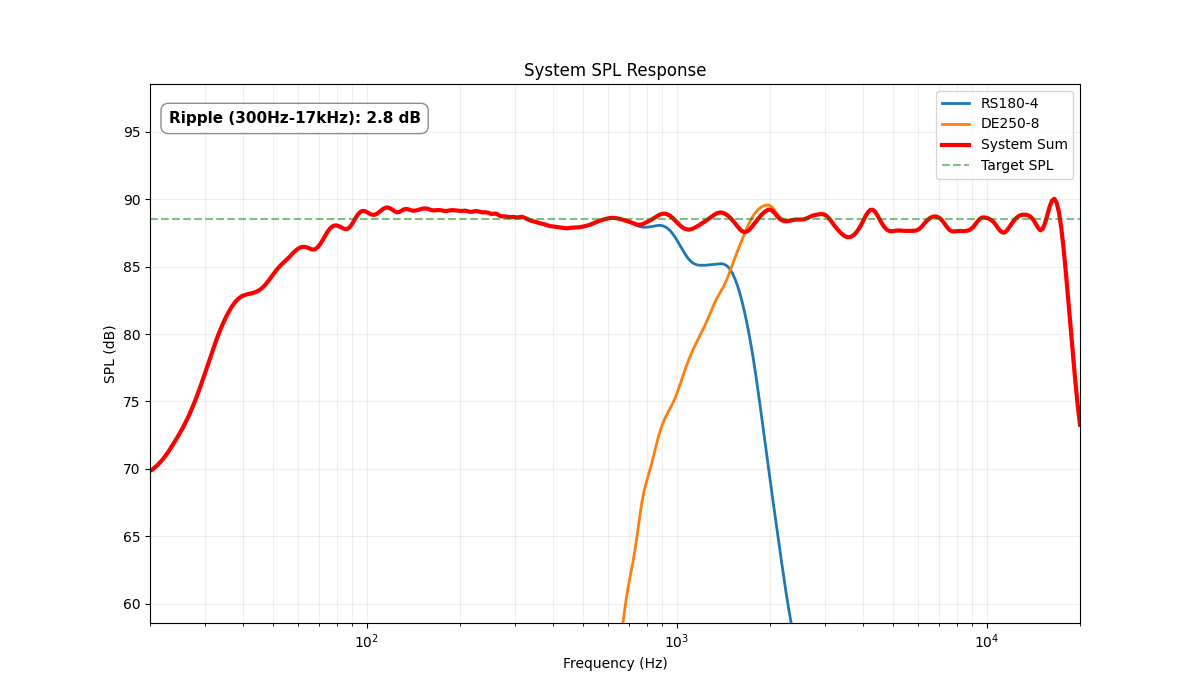
\includegraphics[width=1\linewidth]{RS180-4_X_DE250-8_Reponse_SPL.png}
\end{figure}





\section{Impedance Response}
\begin{figure}[H]
    \centering
    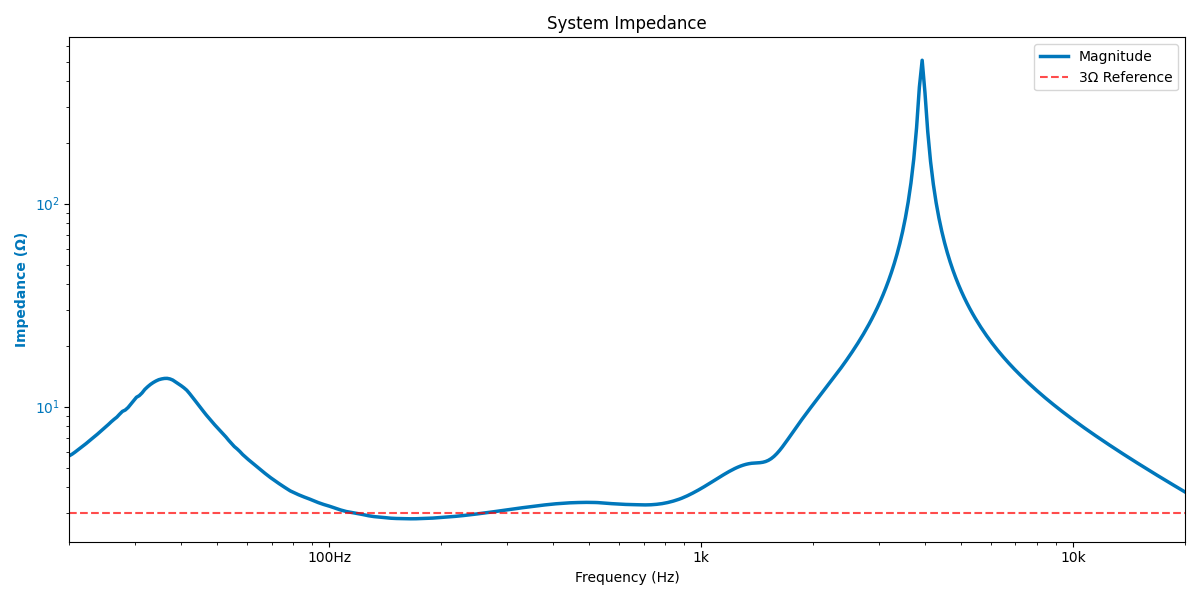
\includegraphics[width=1\linewidth]{RS180-4_X_DE250-8_Impedance.png}
\end{figure}

\chapter{Bill of Materials (BOM)}
The following table lists all the components required to build one crossover. For a stereo pair, please double the quantities. Note that the provided prices and links are for reference only and may vary over time. Always check the supplier's website for the most up-to-date information.

\vspace{0.5cm}
\begin{table}[H]
    \centering
    \renewcommand{\arraystretch}{1.5}
    \begin{tabular}{@{}lllrl@{}}
        \toprule
        \textbf{ID} & \textbf{Component} & \textbf{Value} & \textbf{Price (\$/€)} & \textbf{Buy Link} \\
        \midrule
        C1 & Capacitor & 1.2 $\mu$F & 1.49 & \href{https://www.soundimports.eu/en/jantzen-audio-001-0234.html}{Link} \\
        L1 & Inductor & 0.75 mH & 10.45 & \href{https://www.soundimports.eu/en/jantzen-audio-000-1075.html}{Link} \\
        C2 & Capacitor & 56.0 $\mu$F & 2.95 & \href{https://www.soundimports.eu/en/jantzen-audio-001-6162.html}{Link} \\
        L2 & Inductor & 0.56 mH & 7.45 & \href{https://www.soundimports.eu/en/jantzen-audio-000-2377.html}{Link} \\
        C3 & Capacitor & 40.0 $\mu$F & 9.89 & \href{https://www.parts-express.com/Dayton-Audio-PMPC-40-40uF-250V-Precision-Audio-Capacitor-027-260}{Link} \\
        C4 & Capacitor & 1.2 $\mu$F & 1.49 & \href{https://www.soundimports.eu/en/jantzen-audio-001-0234.html}{Link} \\
        C5 & Capacitor & 5.6 $\mu$F & 0.99 & \href{https://www.parts-express.com/5.6uF-100V-Non-Polarized-Capacitor-027-334}{Link} \\
        R1 & Resistor & 6.5 $\Omega$ & 1.25 & \href{https://www.parts-express.com/Dayton-Audio-DNR-6.5-6.5-Ohm-10W-Precision-Audio-Grade-Resis-004-6.5}{Link} \\
        L3 & Inductor & 0.6 mH & 7.29 & \href{https://www.parts-express.com/Jantzen-1951-0.60mH-18-AWG-Air-Core-Inductor-255-234}{Link} \\
        \midrule
        \multicolumn{3}{r}{\textbf{Estimated Total}} & \textbf{43.25} & \\
        \bottomrule
    \end{tabular}
\end{table}


\chapter{Crossover Design}
This section provides the electrical schematic required to build the crossover and achieve the acoustic results presented earlier. If you need help understanding this diagram, please refer to the beginner guide.

\section{Electrical Schematic}
\begin{figure}[H]
    \centering
    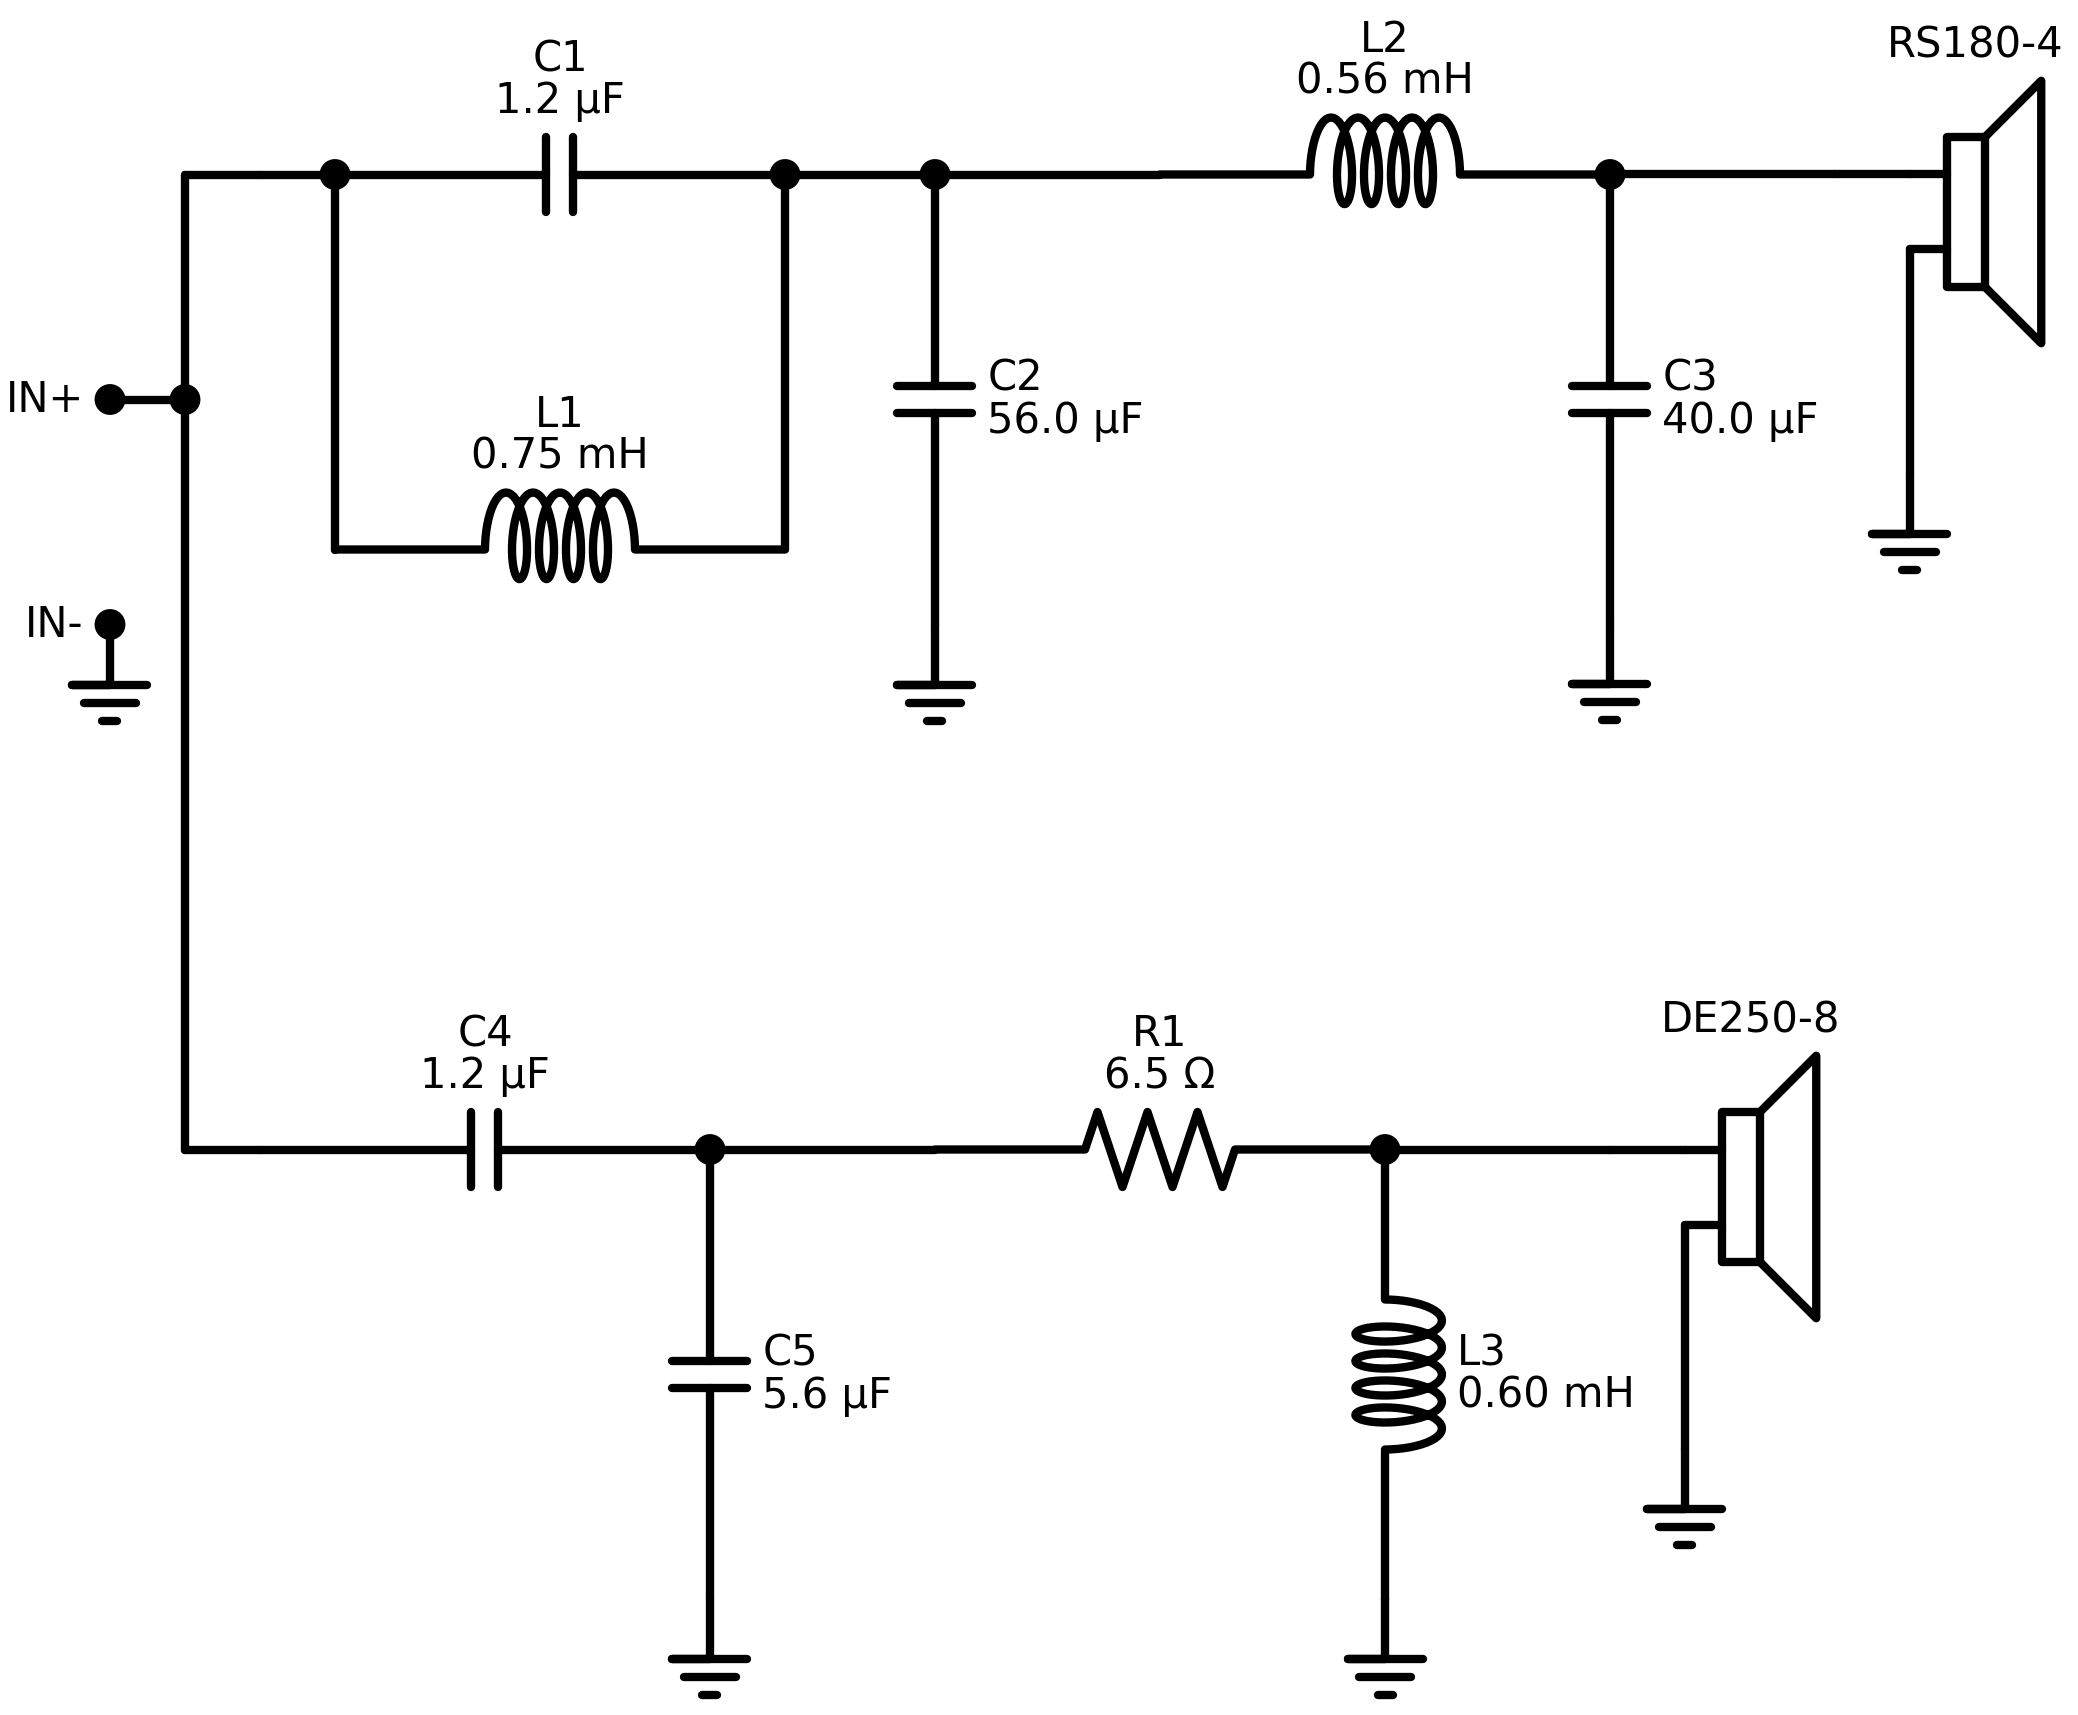
\includegraphics[width=0.8\linewidth]{RS180-4_X_DE250-8_Schema.png}
\end{figure}

\section{Baffle Geometry}
All figures are computed using the following baffle layout. We recommend using this layout for optimal acoustic performance, but feel free to experiment with different placements if you have specific constraints or preferences. 
Just keep in mind that drastically changing the geometry may affect the frequency response and directivity of your speakers due to phase shifts.  
\begin{figure}[H]
    \centering
    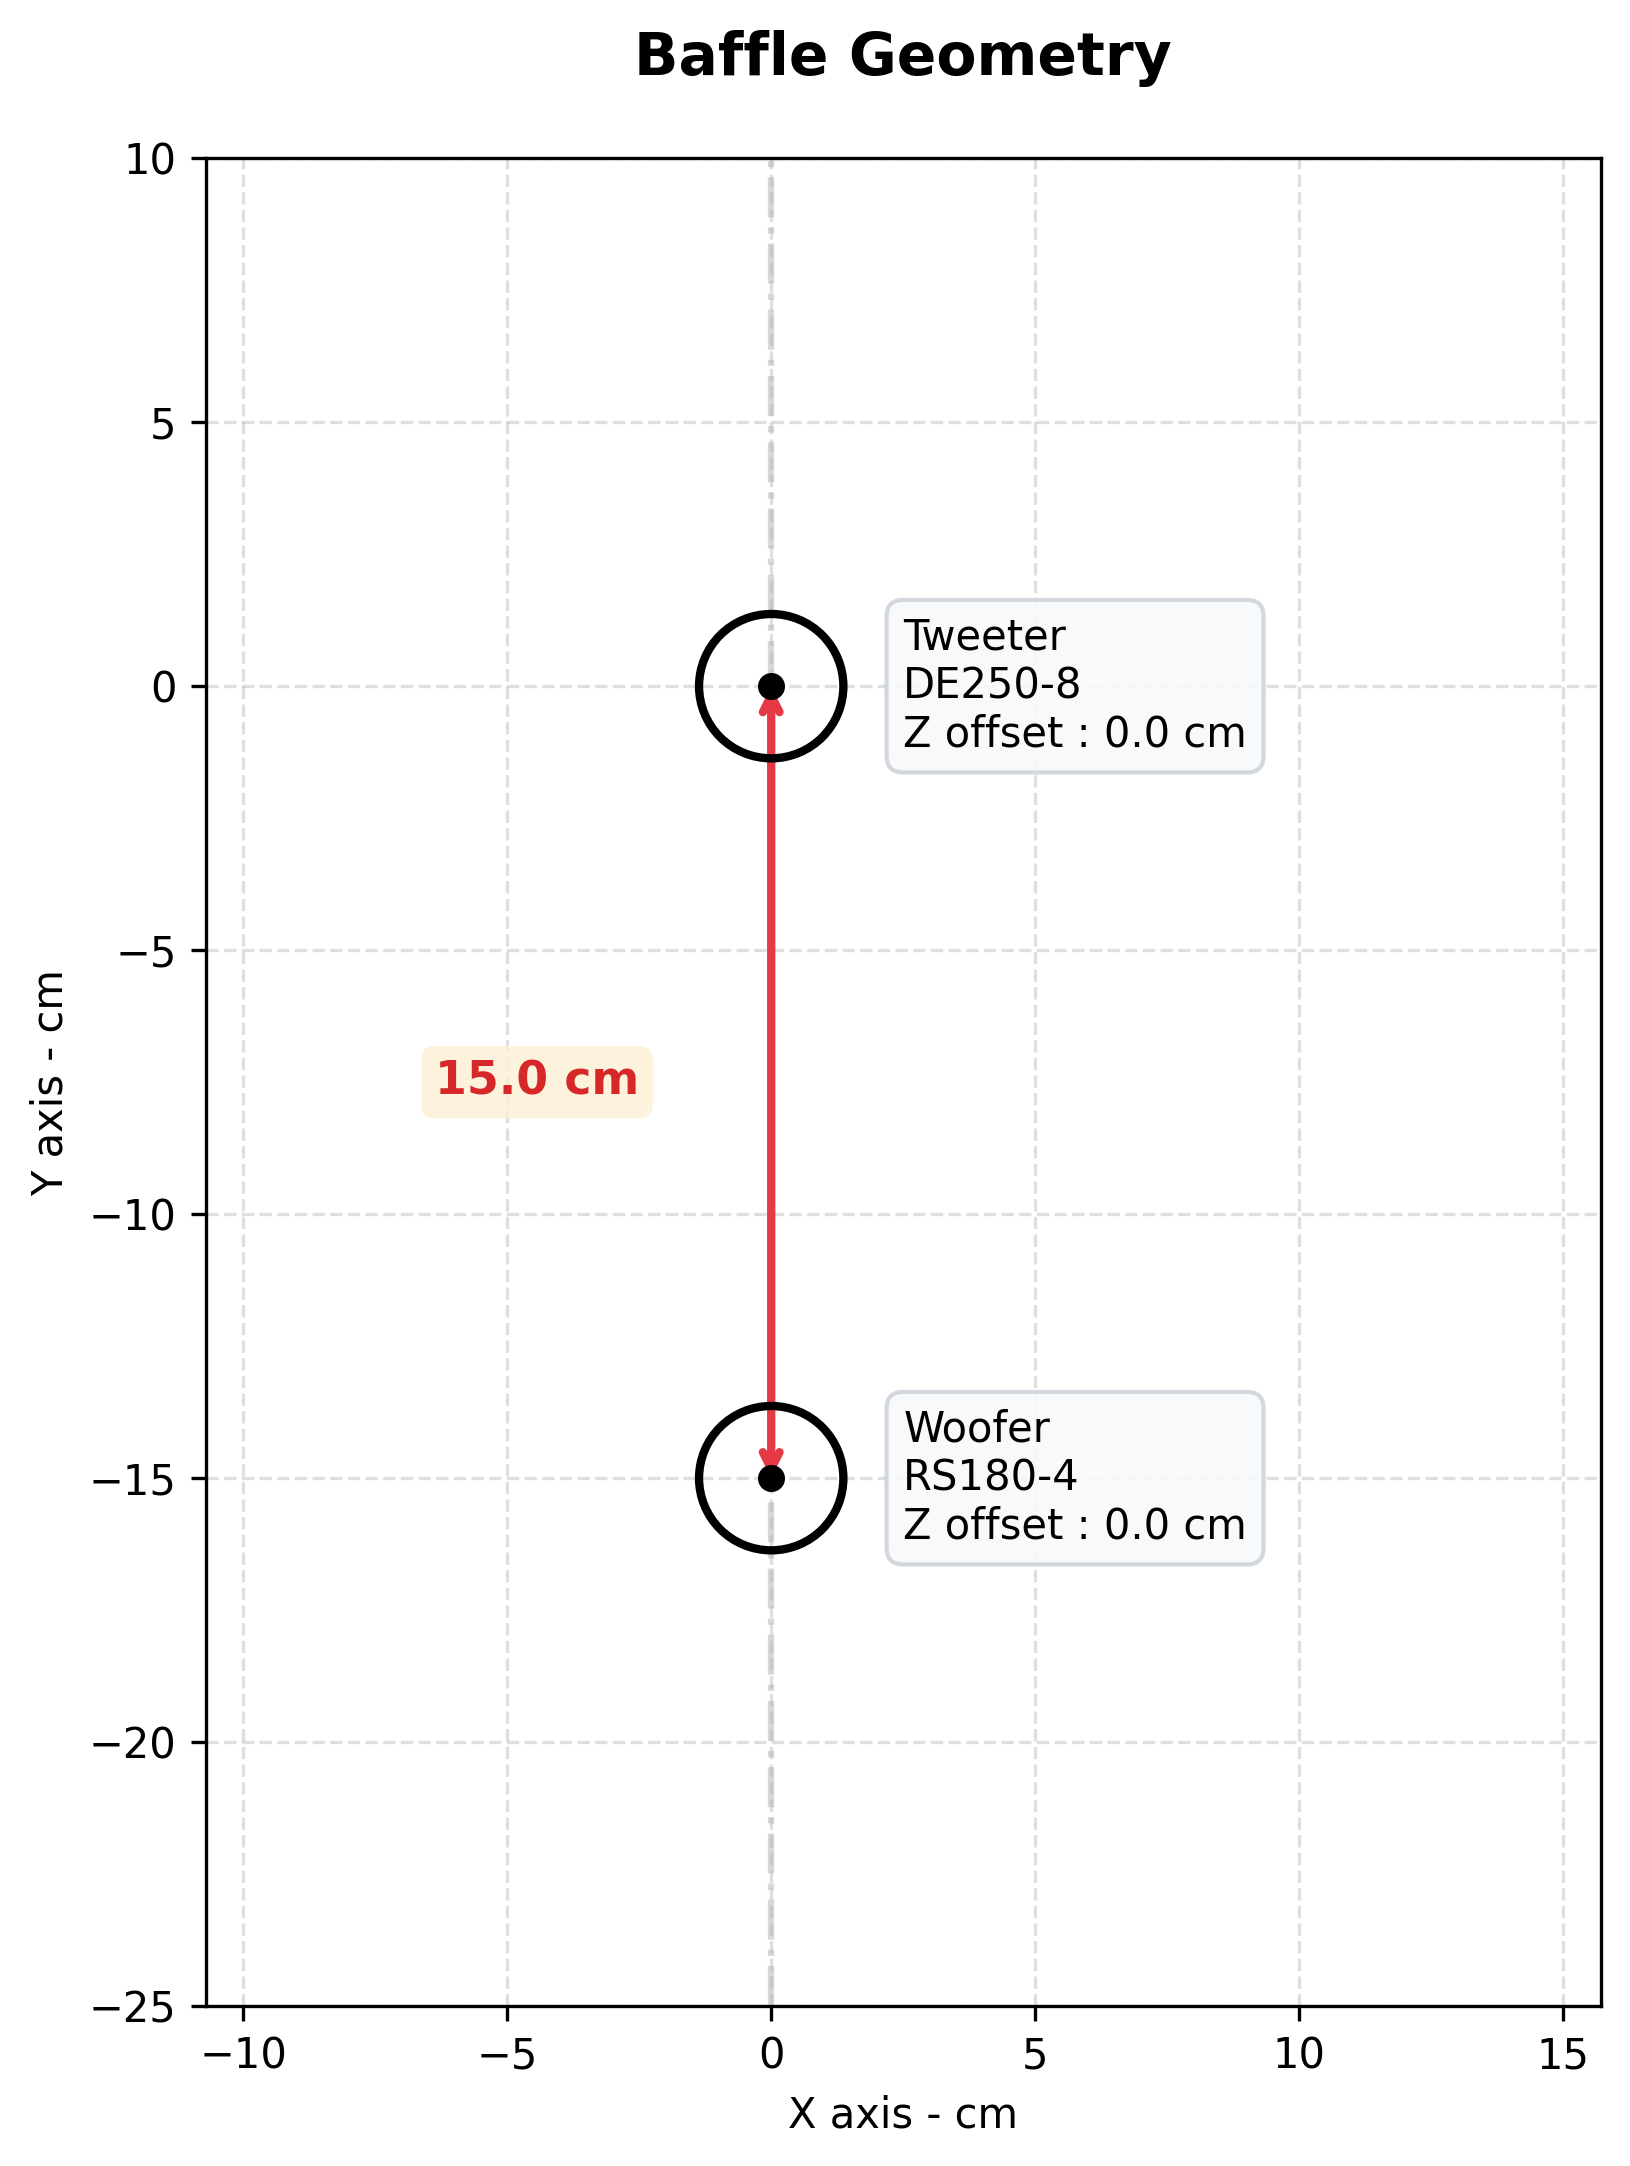
\includegraphics[width=0.80\linewidth]{RS180-4_X_DE250-8_Geometry.png}
\end{figure}

\clearpage
\thispagestyle{empty} 
\begin{tikzpicture}[remember picture,overlay]
    \fill[AudioDark] (current page.north west) rectangle (current page.south east);
    \fill[AudioAccent] ([xshift=1cm]current page.north west) rectangle ([xshift=1.2cm]current page.south west);

    \node[text=white, font=\fontsize{40}{50}\selectfont\bfseries, anchor=west] at ([xshift=2.5cm, yshift=4cm]current page.west) {THANK YOU};
    \node[text=AudioAccent, font=\fontsize{25}{35}\selectfont\bfseries, anchor=west] at ([xshift=2.5cm, yshift=2.5cm]current page.west) {FOR YOUR SUPPORT};

    \node[text=gray, font=\Large, anchor=west, text width=13cm] at ([xshift=2.5cm, yshift=-0.5cm]current page.west) {I hope this guide helps you build the crossover for your DIY audio project. \\ \vspace{0.5cm} If you have any questions, run into issues, or just want to share a picture of your finished build, please feel free to reach out via Etsy messages!};

    \node[text=white, font=\Large\bfseries, anchor=west] at ([xshift=2.5cm, yshift=-4cm]current page.west) {Happy building,};
    \node[text=AudioAccent, font=\Large\bfseries, anchor=west] at ([xshift=2.5cm, yshift=-4.8cm]current page.west) {Audio440};

    % --- INSERTION DU LOGO AVEC CHEMIN ABSOLU ---
    \node[anchor=north west] at ([xshift=2.5cm, yshift=-22cm]current page.north west) {\IfFileExists{C:/Geekosphere/FindMyCrossover/utils/logo.png}{
\includegraphics[width=4cm]{C:/Geekosphere/FindMyCrossover/utils/logo.png}}{}};
    
    \node[text=white, font=\large, anchor=south west] at ([xshift=2.5cm, yshift=2cm]current page.south west) {\href{https://www.etsy.com/shop/Audio440}{www.etsy.com/shop/Audio440}};
\end{tikzpicture}
\end{document}
